% Assignment 1 report, LLM course, Group 9. ACL template, preprint mode (named authors, page numbers).
% Build: pdflatex main && bibtex main && pdflatex main && pdflatex main  (or latexmk -pdf main)
\documentclass[11pt]{article}

\usepackage[preprint]{acl}

\usepackage{times}
\usepackage{latexsym}
\usepackage[T1]{fontenc}
\usepackage[utf8]{inputenc}
\usepackage{microtype}
\usepackage{inconsolata}
\usepackage{graphicx}
\usepackage{booktabs}
\usepackage{amsmath}
\usepackage{amssymb}
\usepackage[capitalise,noabbrev]{cleveref}

% Tighter reference list: no extra space between entries.
\makeatletter
\let\acl@thebibliography\thebibliography
\renewcommand{\thebibliography}[1]{\acl@thebibliography{#1}\setlength{\itemsep}{0pt}\setlength{\parsep}{0pt}}
\makeatother

% Label names. The official tokens are EQUIVALENCE, FORWARD_ENTAILMENT,
% BACKWARD_ENTAILMENT and NEGATIVE_OTHER.
\newcommand{\EQ}{\textsc{Equivalence}}
\newcommand{\FW}{\textsc{Forward}}
\newcommand{\BW}{\textsc{Backward}}
\newcommand{\NO}{\textsc{Negative}}
\newcommand{\Rev}{\operatorname{Rev}}
\newcommand{\SoftCons}{\textsc{SoftCons}}
\newcommand{\HardCons}{\textsc{HardCons}}

\title{How Far Do Surface Cues Go?\\
Baselines for SemEval-2027 Task 2 (DiCo-NLI)}

\author{
  M. Shaheer Saleh \\ 467668 \And
  Ahmad Imran \\ 462852 \And
  Syed Fawwad Ahmed \\ 463933 \And
  Aqib Raza \\ 461312 \AND
  Group 9, Large Language Models course, NUST \\
  \url{https://github.com/Fawwad795/dico-nli-semeval2027-group-9}
}

\begin{document}
\maketitle

\begin{abstract}
SemEval-2027 Task 2 (DiCo-NLI) hands a system two short phrases in a fixed order and asks which of four relations holds between them: equivalence, entailment in either direction, or none. It also checks whether the system's answer on a pair agrees with its answer when the pair is turned around. We wanted to know how much of this a model can get right without reading for meaning at all. On the English track, surface form already gives direction away. In 78\% of forward-entailment training instances the premise is the longer phrase, and in 45\% every word of the hypothesis already appears in the premise. A logistic regression on 17 cues of this kind reaches weighted F1 0.531 on the development set, and it is the most self-consistent of our classical baselines, with \SoftCons{} 0.794. A fine-tuned DeBERTa-v3-base does far better, 0.807 $\pm$ 0.015 weighted F1 over three seeds with \SoftCons{} 0.877 and \HardCons{} 0.810, and its gain comes almost entirely from the instances where length says nothing and from the line between equivalence and entailment. What it still gets wrong are prepositions, numerals and single substituted words. We also note that a system which answers \EQ{} to everything gets a perfect \SoftCons{}, so none of the three official scores means much on its own.
\end{abstract}

\section{Introduction and Task Definition}
\label{sec:intro}

\paragraph{The task as a black box.}
DiCo-NLI \citep{dico-nli-2027-task} gives a system an ordered pair of short phrases, a premise $p$ and a hypothesis $h$, and asks for one of four labels, the set $\mathcal{L}$: \EQ{} (the phrases mean the same), \FW{} ($p$ entails $h$), \BW{} ($h$ entails $p$) or \NO{} (none of these; \cref{tab:task}). It is single-label, four-way classification over ordered pairs. Every reversible source pair appears twice, once in each order, and the gold labels of the two orders are tied by a fixed reversal operator: \EQ{} stays \EQ{}, and \FW{} and \BW{} swap. The organisers report three scores side by side: weighted F1 over all instances, \SoftCons{} (do the system's two answers on a pair obey the reversal operator) and \HardCons{} (are both answers correct); \cref{sec:evaluation} defines them. What a system observes is the two phrase strings and their language codes; the instance and pair identifiers are bookkeeping.

\begin{table}[t]
\centering
\small
\begin{tabular}{@{}p{0.27\columnwidth}p{0.65\columnwidth}@{}}
\toprule
Input & ordered phrase pair $(p, h)$, English, about three words each \\
Output & one label per ordered pair \\
Label space & \EQ, \FW, \BW, \NO \\
Formulation & four-way classification with a cross-instance constraint between $(p,h)$ and $(h,p)$ \\
Official scores & weighted F1, \SoftCons, \HardCons \\
Our data & track 1 (English): train 3,042, dev 660 instances; dev serves as our test set \\
\bottomrule
\end{tabular}
\caption{DiCo-NLI track 1 at a glance.}
\label{tab:task}
\end{table}

\paragraph{The task as a white box.}
Whether one phrase entails another depends on whether its meaning is contained in the other's: in natural logic, adding a restrictive modifier narrows a phrase and yields forward entailment \citep{maccartney-manning-2009-extended}. The relevant cues are therefore which phrase carries extra material, whether the heads match, and what quantifiers, numerals and prepositions do to scope. The same structure invites shortcuts: if the more specific phrase is usually the longer one, length and word containment can predict direction without any semantics, and \cref{sec:eda} shows they do.

Three further confounds matter. The instance identifier leaks the label, since only reversible pairs have a \texttt{\_\_flipped} twin, so no model input may include it. A fifth of the development phrases also occur in training. The source of each pair (image captions or news headlines) is not part of the release.

\paragraph{Why the task is hard.}
The phrases are about three words long and carry no sentence context. Separating equivalence from entailment needs lexical knowledge (``a chocolate bar'' and ``a candy bar''), negatives are often a single substituted word inside an identical frame (``off Mexico'' and ``on Mexico''), and consistency is a property of two predictions that a classifier makes independently.

\paragraph{Question and findings.}
We ask whether systems reach directional consistency by representing the relation between the two phrases or by exploiting surface asymmetries, and how much of a fine-tuned encoder's three scores a cue-only model recovers. We test three hypotheses. H1: a cue-only model reaches a large share of the encoder's \SoftCons{}, because its cues are symmetric or change sign exactly under reversal. H2: the encoder's advantage concentrates where the cues are uninformative, including the boundary between equivalence and entailment. H3: accuracy and consistency trade off in models trained on single ordered instances. H1 and H2 hold; H3 holds inside our classical baselines and fails for the encoder.

\section{Related Work}
\label{sec:related}

\paragraph{The pilot study.}
\citet{apaolaza-larraya-etal-2026-assessing} define the two consistency measures used by the task as soft and hard causal coherence and evaluate encoder, decoder and encoder-decoder transformers on PhrasIS phrase pairs. Each model was tuned with up to 150 Optuna trials on an 80/20 split of the training data. Encoders lead throughout, with DeBERTa-v3-base reaching weighted F1 0.75, soft coherence 0.84 and hard coherence 0.79 on the combined positives track; decoder-only models trail on both accuracy and coherence, and every family loses ground on unseen pairs. Their manual analysis names prepositional phrases and near-synonym or taxonomic relations as the main sources of error. Their positives track has no negatives and uses a different split, so we read these numbers as a reference point and not as a target.

\paragraph{Direction and the reversal curse.}
The task takes its framing from \citet{berglund-etal-2024-reversal}: autoregressive language models fine-tuned on ``A is B'' fail to answer ``B is A''. \citet{lv-etal-2024-analysis} trace the failure to the next-token objective and its causal attention, and repair it at training time. DiCo-NLI is an easier setting, since both phrases are given, but the pilot's decoder results suggest the asymmetry persists. Direction is also fragile in monotonicity reasoning: \citet{yanaka-etal-2019-help} show that NLI models handle upward inferences far better than downward ones, which is the forward and backward distinction at phrase level.

\paragraph{Consistency as a constraint.}
\citet{minervini-riedel-2018-adversarially} and \citet{li-etal-2019-logic} turn logical relations between groups of NLI examples (symmetry of contradiction, transitivity) into training penalties and improve both accuracy and consistency. \citet{elazar-etal-2021-measuring} define consistency as invariance under meaning-preserving rewording and measure it on ParaRel. Reversal is a constraint of the same family, with the difference that the label must change in a prescribed way.

\paragraph{Data and models.}
The phrases come from PhrasIS \citep{lopez-gazpio-etal-2024-phrasis}, which annotates phrase pairs extracted from the chunk alignments of interpretable semantic textual similarity \citep{agirre-etal-2016-semeval-2016}; this origin explains why items are noun phrases, verb chains and prepositional phrases. Our encoder baseline is DeBERTa-v3-base \citep{he-etal-2023-debertav3}, the pilot's strongest base-size model.

\section{Dataset}
\label{sec:dataset}

We use the track 1 (English) training and development files of the official release at commit \texttt{588968e} (8 September 2026). Each reference row holds an instance identifier, a source-pair identifier, the two phrases with language codes, the identifier of its reversed twin and the gold label. \Cref{tab:dataset} gives the split statistics and the quality checks.

\begin{table}[t]
\centering
\footnotesize
\setlength{\tabcolsep}{4pt}
\begin{tabular}{@{}lrr@{}}
\toprule
 & Train & Dev \\
\midrule
Instances & 3,042 & 660 \\
Source pairs & 1,760 & 383 \\
\quad reversible (two instances) & 1,282 & 277 \\
\quad negative (one instance) & 478 & 106 \\
Labels E/F/B/N (\%) & 26/29/29/16 & 26/29/29/16 \\
Words per phrase, mean (max) & 3.0 (15) & 2.9 (10) \\
\midrule
Missing or empty texts & 0 & 0 \\
Duplicate pairs, groups (rows) & 43 (51) & 4 (4) \\
\quad with conflicting labels & 1 & 0 \\
One-word phrases & 563 & 135 \\
Phrases of 8+ words & 27 & 7 \\
Phrases starting with a clitic & 56 & 21 \\
Language pair & en, en & en, en \\
\bottomrule
\end{tabular}
\caption{Track 1 splits and quality checks. E/F/B/N: \EQ, \FW, \BW, \NO. Duplicate rows are extra copies of an ordered pair; phrase counts are occurrences over both sides of every instance; clitic phrases include those starting with punctuation.}
\label{tab:dataset}
\end{table}

\paragraph{Splits.}
The official test set appears only on 10 January 2027, after the course ends, so the development set is our test set. We never select anything on it: model selection uses slices of the training data split by source pair, so that both directions of a pair stay on the same side. Train and dev share no source pair, but 7 unordered phrase pairs and 155 of the 712 distinct development phrases (22\%) also occur in training.

\paragraph{Quality.}
The data is complete, and the one real defect is small: ``South Africans'' and ``South Africa'' appear in training once as \FW{} and once as \NO{}. One-word phrases are common, and phrases such as ``'s war shrine visit'' are fragments of the source chunking. The image-caption versus news-headline origin is absent from the train and dev files; only the 461-pair trial sample records it (244 caption and 217 headline pairs), so we cannot stratify by source.

\section{Exploratory Data Analysis}
\label{sec:eda}

We ran the analysis on the training split only and organised it around six feature groups, each chosen to answer one question about the task (\cref{tab:eda-groups}). We left out lexical-richness measures such as TTR, MTLD and HD-D on purpose: on three-word phrases they are undefined, or they jump around with a single word. The seven figures of the analysis are collected, without captions, in the separate EDA PDF. Two of them appear here.

\begin{table}[t]
\centering
\small
\begin{tabular}{@{}p{0.25\columnwidth}p{0.67\columnwidth}@{}}
\toprule
Group & Question \\
\midrule
Length & Does the longer phrase predict the direction? \\
Readability & Do word and syllable lengths differ by relation? \\
Lexical & Do overlap and containment separate direction, equivalence and negatives? \\
Semantic & Does embedding similarity separate the relations, and can it see direction? \\
Linguistic & Do heads, POS patterns, adjectives and prepositions vary by relation? \\
Task cues & Are quantifiers, negation, numerals and named entities frequent enough to matter? \\
\bottomrule
\end{tabular}
\caption{The six EDA feature groups and the question each answers.}
\label{tab:eda-groups}
\end{table}

\paragraph{Length.}
\textit{Observation.} The premise is the longer phrase in 78\% of \FW{} instances and the hypothesis in 78\% of \BW{} instances. \EQ{} splits almost evenly (36\% premise longer, 29\% equal, 36\% hypothesis longer), and about half of the \NO{} instances (49\%) have the same length on both sides (\cref{fig:length}). \textit{Interpretation.} Direction leaks through form. The entailing phrase is usually the more specific one, and specificity in this data is mostly added words (``in Russia'' against ``in Russian city of Kazan''), so a model can learn direction without touching meaning. \textit{Implication.} Length goes into the cue baseline. Every model also gets scored separately on the instances where length points the wrong way or nowhere (\cref{sec:error}), because those are the ones that tell us whether anything beyond the shortcut was learned.

\begin{figure}[t]
\centering
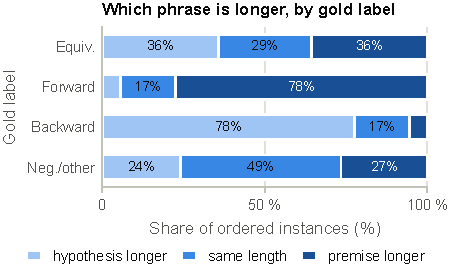
\includegraphics[width=\columnwidth]{figures/eda-length-cue}
\caption{Which phrase is longer, by gold label (train).}
\label{fig:length}
\end{figure}

\paragraph{Lexical overlap and containment.}
\textit{Observation.} Mean word-set Jaccard overlap is 0.41 for directional pairs, against 0.24 for \EQ{} and 0.27 for \NO{}. Containment is one-sided: every hypothesis word occurs in the premise in 45\% of \FW{} instances and only 2\% of \BW{} instances, and the mirror holds for the other direction. The last word is shared in 58\% of directional instances (\cref{fig:lexical}). \textit{Interpretation.} A directional pair is typically one phrase with words added or removed around a head that stays put. Equivalences look different. They are paraphrases, often with little literal overlap: ``Woman and dog'' and ``an adult female accompanied by a dog'' share one word. \textit{Implication.} Containment in both orientations is a strong direction cue when it fires, but it fires on fewer than half of the directional pairs. Overlap tells a model that two phrases are related; it does not tell it that they are equivalent.

\begin{figure*}[t]
\centering
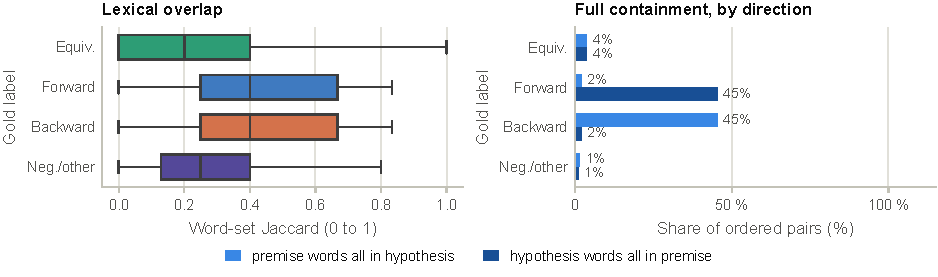
\includegraphics[width=\textwidth]{figures/eda-lexical-containment}
\caption{Word overlap (left) and full containment in each direction (right), by gold label (train).}
\label{fig:lexical}
\end{figure*}

\paragraph{Semantic similarity.}
\textit{Observation.} Cosine similarity of MiniLM sentence embeddings \citep{reimers-gurevych-2019-sentence} has a median of 0.76 for \EQ{}, 0.77 for both directions and 0.64 for \NO{}. 52\% of directional and 50\% of \EQ{} instances sit at or above the \EQ{} median, against 27\% of negatives. Cosine is symmetric, so a pair and its reversal get exactly the same value. \textit{Interpretation.} Similarity separates negatives from related pairs, moderately, and does nothing for the line between \EQ{} and entailment. It carries no information about direction, by construction. \textit{Implication.} We kept cosine out of the cue set. A symmetric representation cannot recover direction, and the equivalence boundary needs something that reads the ordered pair, which is what we expected the encoder to supply.

\paragraph{Linguistic and task-specific cues.}
\textit{Observation.} The two heads share a lemma in 52\% of directional instances against 30\% of \EQ{}. The part-of-speech pattern is identical on both sides in 31\% of \NO{} instances and only 7\% of directional ones. The premise of a \FW{} pair carries 0.33 more adjectives, on average, than its hypothesis. Numerals occur in 18\% of directional instances and named entities in 47\%; quantifiers (3\%) and negation (under 1\%) are rare. \textit{Interpretation.} A negative is often one substituted word inside an unchanged frame (``Two young children'' against ``Two small children'' is labelled \NO{}), and adjectives are the material that narrows a phrase. \textit{Implication.} Comparing heads and modifiers should matter more than any global similarity. Quantifiers and negation are too rare to train on, so we keep them as error-analysis slices instead.

\paragraph{Readability.}
\textit{Observation.} Syllables per word run from 1.53 to 1.60 across labels, characters per word from 4.5 to 4.9, and median Flesch reading ease from 77.9 to 82.4. \textit{Interpretation.} The phrases are uniformly short caption and headline language. Flesch assumes sentences, and on fragments it only tracks syllable density. \textit{Implication.} Readability does not separate the labels and stays out of the feature set. It stays in the report so that nobody has to rerun the check.

\section{Feature Engineering}
\label{sec:features}

The classical baselines use two feature sets, both computed from the two phrase strings only; a unit test checks that no identifier reaches the feature matrix.

\paragraph{Surface cues.}
Seventeen numeric cues turn the EDA findings into features (\cref{tab:cues}). Each cue is either unchanged when the pair is reversed (overlap, shared words) or changes sign or swaps with its partner (length differences, the two containments), which matters for consistency in \cref{sec:results}. Readability and embedding similarity are excluded for the reasons given in \cref{sec:eda}. The cues are standardised on the training data.

\begin{table}[t]
\centering
\small
\begin{tabular}{@{}p{0.30\columnwidth}p{0.62\columnwidth}@{}}
\toprule
Group & Cues \\
\midrule
Length (7) & words and characters per side, their differences, log word ratio \\
Overlap (2) & shared words, Jaccard \\
Containment (4) & share of each side's words in the other; each side contained as a contiguous span \\
Position (2) & same first word, same last word \\
Numerals (2) & a digit on each side \\
\bottomrule
\end{tabular}
\caption{The 17 surface cues, grouped.}
\label{tab:cues}
\end{table}

\paragraph{Lexical n-grams.}
TF-IDF over word unigrams and bigrams of the string ``$p$ \texttt{[SEP]} $h$'', with sublinear term frequency. The token pattern keeps one-letter words and the separator as a token of its own, so bigrams that cross the separator encode which phrase a word belongs to.

\section{Baseline Models}
\label{sec:baselines}

Every setting below was fixed before the first run. Nothing was tuned on the development set.

\paragraph{Trivial systems.}
A majority-label predictor, a uniform random predictor with seed 13, and two constant predictors that answer \EQ{} everywhere and \NO{} everywhere. The majority system has a quirk worth recording: \FW{} and \BW{} tie at 881 training instances each, the tie goes to the first label in canonical order, and so it predicts \FW{} for everything. The two constant systems exist to probe the metrics (\cref{sec:evaluation}).

\paragraph{Classical baselines.}
Logistic regression on the cues, on the n-grams, and on both together, plus gradient-boosted trees on the cues, all in scikit-learn \citep{pedregosa-etal-2011-scikit} with balanced class weights. The regressions use $C = 1$; the trees run 300 iterations at learning rate 0.05; everything else is a library default.

\paragraph{Pretrained baseline.}
DeBERTa-v3-base \citep{he-etal-2023-debertav3} with a classification head, fully fine-tuned with Hugging Face Transformers \citep{wolf-etal-2020-transformers} in a training loop we wrote ourselves so that the seed controls everything. The pair is tokenised as one sequence of at most 32 tokens. Training runs 5 epochs of AdamW at learning rate $2 \times 10^{-5}$, batch size 16, weight decay 0.01, a linear schedule with 6\% warm-up and gradient clipping at 1.0, and we keep the epoch with the best weighted F1 on a 20\% slice of the training data, again split by source pair. Three seeds (13, 42, 1234), each drawing its own slice. One detail tripped us up: under Transformers 5 the checkpoint loads in float16, and the first GPU epoch trained with a NaN loss from its first step until we forced float32. After that, each run trained in about 140 seconds on one NVIDIA T4, and a second execution reproduced every development prediction exactly.

\section{Evaluation Setup}
\label{sec:evaluation}

\paragraph{Weighted F1.}
With $n_c$ gold instances of label $c$ among $N$, and $F_c$ the F1 of label $c$,
\begin{equation}
\text{wF1} = \sum_{c \in \mathcal{L}} \frac{n_c}{N} F_c, \qquad F_c = \frac{2 P_c R_c}{P_c + R_c}.
\end{equation}
Each label counts in proportion to how often it occurs. So \NO{}, 16\% of the data and the hardest class for every one of our models, weighs the least. That is why we print macro F1, which averages the $F_c$ with equal weights, next to the official score: a weak minority class should stay visible. Micro F1 would equal accuracy here, since every instance has exactly one label.

\paragraph{Consistency.}
Let $\Rev$ map \EQ{} to \EQ{}, \FW{} to \BW{} and \BW{} to \FW{}; \NO{} has no reverse. Let $\mathcal{P}$ be the set of reversible pairs $(x, x^{r})$ in the development set ($|\mathcal{P}| = 277$), $f$ the system, $y$ the gold label and $\mathbb{I}[\cdot]$ the indicator:
\begingroup\small
\begin{align}
\SoftCons &= \frac{1}{|\mathcal{P}|} \sum_{\mathcal{P}} \mathbb{I}\big[f(x) = \Rev(f(x^{r}))\big], \\
\HardCons &= \frac{1}{|\mathcal{P}|} \sum_{\mathcal{P}} \mathbb{I}\big[f(x) = y \wedge f(x^{r}) = y^{r}\big].
\end{align}
\endgroup
Since the gold labels obey the reversal themselves, a pair that is right in both directions is automatically consistent, so $\HardCons \le \SoftCons$ always. Negative pairs have no reversed twin and enter weighted F1 only. A \NO{} prediction on a reversible pair counts as incompatible.

\paragraph{What each score rewards.}
Weighted F1 rewards correct labels on single instances. \SoftCons{} rewards agreeing with yourself, right or wrong. \HardCons{} rewards being right on whole pairs. The constant systems make the difference concrete. Answer \EQ{} everywhere and you are consistent on every single pair: \SoftCons{} 1.000, weighted F1 0.110, and a \HardCons{} of 0.314 that is simply the share of reversible pairs whose gold label is \EQ{} (87 of 277). Answer \NO{} everywhere and you get 0.044, 0 and 0. Neither system knows anything. This is why we never quote one of the three scores on its own.

\paragraph{Protocol.}
Every score comes from the official scorer, run unchanged, the way the competition platform runs it. The classical baselines are also cross-validated on the training data, five folds grouped by source pair, each fold scored by the same scorer. Each run records its seed, the data commit, the code commit and the exact command, and \cref{app:runs} maps every number in this report back to its run folder.

\section{Results}
\label{sec:results}

\Cref{tab:results} lists every system on the development set. Cross-validation on the training data ranks the classical systems in the same order as the development set. Every development score is at or below its cross-validated mean, by 0.1 to 1.2 standard deviations and by 2.0 for n-grams alone, so the development set is somewhat harder than held-out training folds.

\begin{table*}[t]
\centering
\footnotesize
\setlength{\tabcolsep}{3.5pt}
\begin{tabular}{@{}lccccc@{}}
\toprule
System & Weighted F1 & Macro F1 & \SoftCons & \HardCons & CV weighted F1 \\
\midrule
Majority (\FW{} everywhere) & 0.129 & 0.112 & 0.000 & 0.000 & \\
Random, seed 13 & 0.246 & 0.240 & 0.184 & 0.054 & \\
\EQ{} everywhere & 0.110 & 0.104 & 1.000 & 0.314 & \\
\NO{} everywhere & 0.044 & 0.069 & 0.000 & 0.000 & \\
\midrule
Cues, logistic regression & 0.531 & 0.502 & 0.794 & 0.552 & 0.575 $\pm$ 0.037 \\
N-grams, logistic regression & 0.407 & 0.399 & 0.426 & 0.256 & 0.429 $\pm$ 0.011 \\
Cues and n-grams, logistic regression & 0.596 & 0.573 & 0.747 & 0.570 & 0.617 $\pm$ 0.021 \\
Cues, gradient-boosted trees & 0.574 & 0.550 & 0.718 & 0.527 & 0.572 $\pm$ 0.024 \\
\midrule
DeBERTa-v3-base, mean $\pm$ sd of 3 seeds & \textbf{0.807} $\pm$ 0.015 & \textbf{0.786} $\pm$ 0.017 & \textbf{0.877} $\pm$ 0.010 & \textbf{0.810} $\pm$ 0.013 & \\
\midrule
\textit{Pilot DeBERTa-v3-base, other track$^{\dagger}$} & \textit{0.75} & \textit{n/a} & \textit{0.84} & \textit{0.79} & \\
\bottomrule
\end{tabular}
\caption{Track 1 development set, official scorer. CV: cross-validation on the training data, five folds grouped by source pair, mean $\pm$ sd. For DeBERTa the held-out weighted F1 at the selected epoch averages 0.798. $^{\dagger}$Reported by \citet{apaolaza-larraya-etal-2026-assessing} on the PhrasIS positives track, without negatives and on another split; a reference point, not comparable.}
\label{tab:results}
\end{table*}

\paragraph{Surface cues buy consistency (H1).}
The cue-only model is the most self-consistent classical system: 220 of the 277 reversible pairs get compatible answers, and it confuses \FW{} with \BW{} in only 8 of the 380 directional instances. Its weights follow the EDA (\cref{tab:weights}): hypothesis-in-premise containment pushes towards \FW{} and away from \BW{}, its mirror does the reverse, and the length differences add a smaller push of the same kind. Because these cues swap or change sign under reversal, the model's decisions on a pair and its reversal are compatible almost by construction. Consistency is not correctness, though: 67 of its 220 consistent pairs are wrong in both directions, so \HardCons{} stays at 0.552.

\begin{table}[t]
\centering
\footnotesize
\setlength{\tabcolsep}{5pt}
\begin{tabular}{@{}lrrrr@{}}
\toprule
Cue & E & F & B & N \\
\midrule
$h$ words in $p$ & $-0.09$ & $+0.96$ & $-1.44$ & $+0.57$ \\
$p$ words in $h$ & $-0.02$ & $-1.35$ & $+0.97$ & $+0.41$ \\
Jaccard overlap & $-0.42$ & $+0.84$ & $+0.82$ & $-1.25$ \\
Character difference & $+0.01$ & $+0.49$ & $-0.49$ & $-0.01$ \\
Log word ratio & $-0.02$ & $+0.39$ & $-0.38$ & $+0.02$ \\
\bottomrule
\end{tabular}
\caption{The five largest standardised weights of the cue-only logistic regression, per label (E/F/B/N: \EQ, \FW, \BW, \NO).}
\label{tab:weights}
\end{table}

\paragraph{Inside the classical family, accuracy costs consistency (H3).}
Adding n-grams to the cues raises weighted F1 from 0.531 to 0.596 and lowers \SoftCons{} from 0.794 to 0.747; trees on the same cues show the same trade (0.574 and 0.718). The more expressive models find order-specific patterns that help single instances and break agreement across the pair. N-grams alone see the order only through bigrams that cross the separator, and score lowest on every metric.

\paragraph{The encoder gains on all three (H3 fails for it).}
DeBERTa-v3-base raises weighted F1 by 0.21 and \HardCons{} by 0.24 over the best classical system, and \SoftCons{} by 0.08 over the most consistent one (\cref{fig:tradeoff}). The gain is largest where the cues were weakest: against the combined classical model, F1 on \EQ{} rises from 0.45 to 0.78 and on \NO{} from 0.41 to 0.63, while the two directions rise from 0.72 and 0.71 to 0.86 and 0.87. Its consistency follows from correctness: only 16 to 21 of its consistent pairs per seed are wrong. We do not claim it beats the pilot, whose numbers come from another track, another split and a 150-trial search.

\begin{figure}[t]
\centering
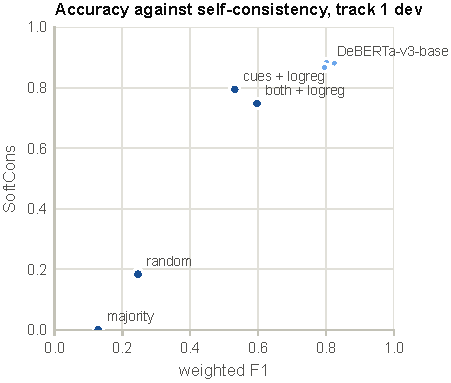
\includegraphics[width=\columnwidth]{figures/results-f1-vs-softcons}
\caption{Weighted F1 against \SoftCons{} on the development set; small points are the three DeBERTa seeds.}
\label{fig:tradeoff}
\end{figure}

\section{Error Analysis}
\label{sec:error}

\paragraph{How pairs fail.}
\Cref{tab:pairs} sorts each reversible development pair by what a system did with its two directions. The cue model almost never gets one direction right and the other wrong (1 pair): its errors are symmetric, either consistent and wrong (67) or wrong both ways (56). Adding n-grams turns 21 pairs into half-right ones, the order-specific behaviour behind its lower \SoftCons{}. DeBERTa leaves 49 to 56 pairs not fully correct per seed, spread evenly over the three failure types.

\begin{table}[t]
\centering
\footnotesize
\setlength{\tabcolsep}{3pt}
\begin{tabular}{@{}lrrrr@{}}
\toprule
 & \multicolumn{2}{c}{Consistent} & \multicolumn{2}{c}{Inconsistent} \\
\cmidrule(lr){2-3} \cmidrule(l){4-5}
System & right & wrong & one right & both wrong \\
\midrule
Cues & 153 & 67 & 1 & 56 \\
Cues and n-grams & 158 & 49 & 21 & 49 \\
DeBERTa, seed 13 & 228 & 16 & 15 & 18 \\
DeBERTa, seed 42 & 224 & 21 & 12 & 20 \\
DeBERTa, seed 1234 & 221 & 19 & 17 & 20 \\
\bottomrule
\end{tabular}
\caption{Outcomes on the 277 reversible development pairs. A consistent pair is either right in both directions or wrong in both.}
\label{tab:pairs}
\end{table}

\paragraph{Where the encoder wins (H2).}
We split the development instances by what the length cue says about the gold label (\cref{tab:slices}). It agrees on 282 instances, points the wrong way on 10, and says nothing on 368 (equal length, or a label without direction). Where it agrees, the cue model is already strong and the encoder adds 0.02 weighted F1. Where it says nothing, the cue model falls to 0.31 and the encoder holds 0.75, a gap of 0.44.

The misleading slice is too small to read. Slice scores are classification scores only, since a slice can separate the two directions of a pair.

\begin{table}[t]
\centering
\footnotesize
\setlength{\tabcolsep}{4pt}
\begin{tabular}{@{}lrrrr@{}}
\toprule
Length cue & $n$ & Cues & Cues + n-grams & DeBERTa \\
\midrule
Agrees & 282 & 0.907 & 0.917 & 0.931 \\
Misleads & 10 & 0.000 & 0.000 & 0.800 \\
Uninformative & 368 & 0.313 & 0.425 & 0.754 \\
\bottomrule
\end{tabular}
\caption{Weighted F1 on development slices defined by the length cue; DeBERTa is the mean of three seeds.}
\label{tab:slices}
\end{table}

\paragraph{What the encoder still gets wrong.}
DeBERTa rarely confuses direction: seed 13 swaps \FW{} and \BW{} on 3 instances. Its errors sit on the \EQ{} and \NO{} boundaries: 26 directional instances predicted as \EQ{}, 19 \EQ{} instances predicted as \NO{}, and 34 of 106 negatives called related. All three seeds miss the same 80 instances, and the cue model misses 50 of those too. We read 20 hand-picked errors of seed 13 and sorted them into five categories modelled on the pilot's manual analysis (\cref{tab:categories}); the counts are four per category by construction, so they illustrate the kinds of error and do not estimate their rates.

\begin{table*}[t]
\centering
\small
\begin{tabular}{@{}lllll@{}}
\toprule
Category & Premise & Hypothesis & Gold & Predicted \\
\midrule
Preposition & at a pool & in front of a pool & \BW & \NO \\
Numeral or quantifier & A group of people & Six people & \FW & \EQ \\
Near-synonym or taxonomy & a chocolate bar & a candy bar & \FW & \EQ \\
One-word negative contrast & on a crowded street & on a public street & \NO & \EQ \\
Chunking fragment & in destroying & destroy & \FW & \EQ \\
\bottomrule
\end{tabular}
\caption{One example per error category, DeBERTa seed 13 on the development set.}
\label{tab:categories}
\end{table*}

\paragraph{Some errors may be in the gold labels.}
``two people'' and ``2'' are labelled \NO{}, and ``Saudi Women'' to ``Saudis'' is labelled \BW{} although the first phrase is the more specific one; with the conflicting ``South Africans'' duplicate in training (\cref{sec:dataset}), this suggests a share of the remaining errors are annotation disagreements. We have not audited the labels systematically.

\section{Discussion}
\label{sec:discussion}

\paragraph{Direction is the easy part.}
Seventeen surface cues decide \FW{} against \BW{} almost as reliably as a fine-tuned encoder: 8 confusions against 3, out of 380. What the cues cannot decide is the kind of relation. Does the added material narrow the meaning or paraphrase it? Does a swapped word break the relation or keep it? That is where most of the encoder's 0.21 gain in weighted F1 comes from (\cref{tab:slices}), and it is also where the encoder's own errors remain.

\paragraph{\SoftCons{} on its own is easy to game.}
A constant \EQ{} predictor scores a perfect 1.000. The cue model reaches 0.794 while being wrong in both directions on a quarter of the pairs. A system can be consistent by construction, through symmetric or sign-flipping inputs, without any grasp of the relation. We therefore read \SoftCons{} only next to \HardCons{} and macro F1, and we count the consistent-but-wrong pairs explicitly. We would suggest other participants do the same.

\paragraph{The encoder is consistent because it is correct.}
The trade between accuracy and consistency that we saw inside the classical family did not carry over. DeBERTa improved all three scores at once, and almost all of its consistent pairs are correct ones. For decoder models, which the pilot found far less coherent, this sharpens the question for Assignment 2: their consistency gap may be a correctness gap on the hard relations, and not a separate defect that needs its own fix.

\paragraph{How far the numbers travel.}
The development set is a little harder than held-out training folds, a fifth of its phrases also occur in training, and some gold labels look questionable. Differences of a few points between systems should be read with all of that in mind. The differences we draw conclusions from are 0.2 or more.

\section{Next Steps}
\label{sec:next}

Assignment 2 moves to decoder language models, where the pilot found the largest consistency gap. We plan to compare open-weight instruction-tuned models used by prompting and fine-tuned with low-rank adapters, and to test three ways of giving a model direction: training on both orders of every pair, a loss term that penalises incompatible predictions on a pair and its reversal in the manner of \citet{li-etal-2019-logic}, and prompts that show both orders at once. Every system will be reported with weighted F1, macro F1, \SoftCons{}, \HardCons{}, the consistent-but-wrong count and the length-cue slices of \cref{tab:slices}, against the baselines in this report. Before we lean on the error categories any further we will audit the conflicting and questionable gold labels. The Spanish and Basque tracks come in if time allows.

\section*{Limitations}

All results are on one track, English, and on the development set, which we use as a test set because the official test set is not yet released. The classical baselines use one seed and fixed settings, and the encoder three seeds with a fixed recipe; neither was tuned, so the numbers are baselines and not upper bounds. The misleading length-cue slice has 10 instances. The error categories come from 20 hand-picked errors and describe kinds of failure, not their frequency. The part-of-speech and similarity features rely on spaCy's small English model and on one sentence encoder, both applied to phrases without context.


\bibliography{references}

\appendix
\section{Where Every Number Comes From}
\label{app:runs}

\raggedright
Each run folder under \texttt{experiments/} holds a \texttt{config.json} with the seed, the data commit (\texttt{588968e}), the code commit and the exact command, together with the official scorer's report for every system. The notebooks under \texttt{notebooks/assignment-1/} rerun headlessly with \texttt{uv run jupyter execute}; the encoder was trained by the Modal launcher \texttt{scripts/modal/train\_encoder.py} and its outputs fetched before scoring.

\begin{itemize}
\setlength{\itemsep}{2pt}
\small
\item Data checks and EDA: notebook \texttt{02\_eda\_track1}, folder \texttt{2026-09-29-eda-track1}.
\item Trivial and constant systems: notebook \texttt{01\_trivial\_baselines}, folder \texttt{2026-09-29-trivial-baselines-track1}.
\item Classical baselines: notebook \texttt{03\_ml\_baseline\_track1}, folder \texttt{2026-09-29-ml-baseline-track1}.
\item DeBERTa-v3-base: notebook \texttt{04\_dl\_baseline\_track1}, folder \texttt{2026-09-29-deberta-base-track1}.
\item Error analysis: notebook \texttt{05\_error\_analysis\_track1}, folder \texttt{2026-10-02-error-analysis-track1}.
\end{itemize}


\end{document}
